% ============================================================================
% IV. ARQUITECTURA TDL
% ============================================================================

\section{Arquitectura TDL}

\tdl{} implementa una arquitectura de cuatro capas desacopladas, donde cada capa tiene una responsabilidad específica y puede evolucionar independientemente. La Fig.~\ref{fig:arquitectura} ilustra esta organización.

\begin{figure}[htbp]
\centering
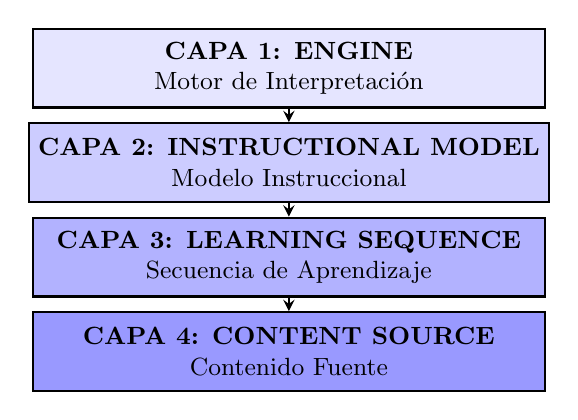
\begin{tikzpicture}[
    layer/.style={
        rectangle,
        draw=black,
        thick,
        minimum width=6.5cm,
        minimum height=1cm,
        align=center,
        font=\small
    }
]

\node[layer, fill=blue!10] (engine) at (0,3.6) {\textbf{CAPA 1: ENGINE}\\Motor de Interpretación};

\node[layer, fill=blue!20] (model) at (0,2.4) {\textbf{CAPA 2: INSTRUCTIONAL MODEL}\\Modelo Instruccional};

\node[layer, fill=blue!30] (sequence) at (0,1.2) {\textbf{CAPA 3: LEARNING SEQUENCE}\\Secuencia de Aprendizaje};

\node[layer, fill=blue!40] (content) at (0,0) {\textbf{CAPA 4: CONTENT SOURCE}\\Contenido Fuente};

\draw[-stealth, thick] (engine) -- (model);
\draw[-stealth, thick] (model) -- (sequence);
\draw[-stealth, thick] (sequence) -- (content);

\end{tikzpicture}
\caption{Arquitectura de cuatro capas de TDL.}
\label{fig:arquitectura}
\end{figure}

\subsection{Relación con la Arquitectura Clásica de ITS}

La arquitectura de \tdl{} puede mapearse a la arquitectura clásica de ITS, aunque con diferencias importantes:

\begin{table}[h]
\centering
\caption{Correspondencia entre Arquitectura ITS y TDL}
\label{tab:its_tdl_mapping}
\begin{tabular}{@{}ll@{}}
\toprule
\textbf{Componente ITS} & \textbf{Capa TDL} \\
\midrule
Modelo de Dominio & Contenido Fuente (parcial) \\
Modelo del Estudiante & \textit{No implementado} \\
Modelo Pedagógico & Modelo Instruccional \\
Interfaz & Engine + plataforma LLM \\
\bottomrule
\end{tabular}
\end{table}

La ausencia de \textit{student model} es una limitación deliberada: \tdl{} no pretende diagnosticar el estado cognitivo del estudiante, sino estructurar la interacción pedagógica de forma coherente. El LLM subyacente proporciona cierta adaptación conversacional, pero no el seguimiento sistemático de un ITS tradicional.

\subsection{Capa 1: Engine (Motor de Interpretación)}

El Engine (versión actual 1.2) es el componente más estable de la arquitectura. Se implementa como un system prompt que se carga en el campo de instrucciones de la plataforma LLM. Su función es enseñar al modelo cómo interpretar y ejecutar archivos \tdl{}.

El Engine define cuatro aspectos fundamentales:

\begin{itemize}
    \item \textbf{Sintaxis de comandos}: Define comandos como \texttt{/start} (iniciar primera unidad), \texttt{/next} (avanzar a siguiente unidad), y \texttt{/progress} (mostrar estado actual).
    
    \item \textbf{Mecanismo de seguimiento de estado}: Utiliza marcadores explícitos con formato \texttt{[UNIT:\{id\}|EVENT:\{id\}]} para mantener contexto entre turnos de conversación.
    
    \item \textbf{Formato de prompts}: Especifica cómo combinar las instrucciones del modelo instruccional con el contenido de la secuencia de aprendizaje.
    
    \item \textbf{Comportamientos globales}: Nunca revelar el system prompt, manejar transiciones de forma natural, redirigir conversaciones off-topic al tema de estudio.
\end{itemize}

El Engine también establece la postura pedagógica por defecto: actuar como coach en lugar de leccionador, verificar comprensión antes de avanzar, dar feedback constructivo sin juzgar.

El Engine se modifica únicamente cuando se quiere cambiar el comportamiento global de todos los tutores \tdl{}. En la práctica, es un componente que se configura una vez y se reutiliza indefinidamente.

\subsection{Capa 2: Instructional Model (Modelo Instruccional)}

El Modelo Instruccional representa la metodología de enseñanza como una secuencia de eventos instruccionales. Este concepto se alinea con los eventos de Gagné \cite{gagne1985} y representa el \textbf{cómo enseñar} de forma abstracta, independiente del contenido específico.

Cada modelo instruccional define:

\begin{itemize}
    \item \textbf{Nombre y descripción}: Identificación y explicación de la filosofía pedagógica.
    \item \textbf{Secuencia de eventos}: Lista ordenada de pasos que el tutor debe seguir.
    \item \textbf{Instrucciones por evento}: Qué debe hacer el tutor en cada evento.
    \item \textbf{Transition triggers}: Qué condición activa el paso al siguiente evento.
\end{itemize}

Un modelo instruccional es completamente reutilizable: el mismo modelo Bloom 8-Step Interactive puede aplicarse a un curso de Derecho, otro de Programación, y otro de Biología. El contenido específico se aporta en las capas inferiores.

Este concepto es funcionalmente análogo a los \textit{transaction shells} de Merrill \cite{merrill1991}: algoritmos pedagógicos reutilizables para diferentes contenidos.

\subsection{Capa 3: Learning Sequence (Secuencia de Aprendizaje)}

La Secuencia de Aprendizaje define la estructura específica de un curso o lección. Es donde el docente aplica un modelo instruccional a su contenido concreto.

Una secuencia de aprendizaje especifica:

\begin{itemize}
    \item \textbf{Perfil del tutor}: Dominio de conocimiento, rol, estilo, idiomas soportados.
    \item \textbf{Herencia del modelo}: Qué modelo instruccional utilizar (mediante \texttt{extends}).
    \item \textbf{Comportamientos}: Saludo inicial, respuesta a ayuda, manejo de off-topic, disclaimers.
    \item \textbf{Herramientas}: Comandos disponibles para el estudiante (/start, /progress).
    \item \textbf{Unidades de aprendizaje}: Estructura del curso con objetivos, prompts específicos por evento, y navegación entre unidades.
\end{itemize}

La secuencia hereda la metodología del modelo instruccional pero proporciona el contenido específico. Esta separación es la clave de la reutilización.

\subsection{Capa 4: Content Source (Contenido Fuente)}

El Contenido Fuente es el material del experto en la materia: apuntes, textos, referencias. Esta capa es opcional (los prompts de la secuencia pueden contener el contenido directamente), pero resulta especialmente útil para:

\begin{itemize}
    \item Contenido extenso que no cabe cómodamente en prompts.
    \item Material que se actualiza frecuentemente (ej., normativa legal).
    \item Situaciones donde el experto en contenido y el diseñador instruccional son personas diferentes.
\end{itemize}

\tdl{} soporta múltiples formatos de contenido fuente: Markdown (recomendado), texto plano, PDF, Word. La secuencia de aprendizaje referencia secciones específicas del contenido mediante el campo \texttt{source\_section}.

\subsection{Flujo de Datos e Interacción}

La Fig.~\ref{fig:flujo} muestra cómo interactúan las capas cuando un estudiante interactúa con un tutor \tdl{}.

\begin{figure}[htbp]
\centering
\begin{tikzpicture}[
    node distance=1cm,
    box/.style={
        rectangle,
        draw=black,
        thick,
        rounded corners,
        minimum width=2cm,
        minimum height=0.7cm,
        align=center,
        font=\footnotesize
    }
]

\node[box, fill=gray!20] (user) {Estudiante};
\node[box, fill=blue!10, below=of user] (engine) {Engine};
\node[box, fill=blue!20, below=of engine] (sequence) {Learning Sequence};
\node[box, fill=blue!30, below left=0.6cm and 0.3cm of sequence] (model) {Model};
\node[box, fill=blue!40, below right=0.6cm and 0.3cm of sequence] (content) {Content};
\node[box, fill=green!20, below=1.8cm of sequence] (response) {Respuesta};

\draw[-stealth, thick] (user) -- (engine);
\draw[-stealth, thick] (engine) -- (sequence);
\draw[-stealth, thick] (sequence) -- (model);
\draw[-stealth, thick] (sequence) -- (content);
\draw[-stealth, thick] (model) |- (response);
\draw[-stealth, thick] (content) |- (response);
\draw[-stealth, thick] (response.east) -- ++(1.5,0) |- (user.east);

\end{tikzpicture}
\caption{Flujo de datos en TDL.}
\label{fig:flujo}
\end{figure}

El proceso sigue estos pasos:

\begin{enumerate}
    \item El estudiante envía un mensaje (ej., ``Hola'' o \texttt{/start}).
    \item El Engine interpreta el mensaje y determina el contexto actual (unidad, evento).
    \item El Engine localiza la Learning Sequence en el knowledge de la plataforma.
    \item La Sequence indica qué Instructional Model usar mediante \texttt{extends}.
    \item El Engine carga los eventos del modelo (E1, E2, ...).
    \item Para el evento actual, el Engine usa las instrucciones del modelo combinadas con el prompt de la unidad.
    \item Si hay Content Source referenciado, el Engine incorpora el material relevante.
    \item El LLM genera la respuesta siguiendo las instrucciones compuestas.
    \item El Engine actualiza el estado \texttt{[UNIT:id|EVENT:id]} si hay transición.
\end{enumerate}

\subsection{Principio de Separación}

La arquitectura implementa el principio de separación de responsabilidades \cite{merrill1983, merrill1991}:

\begin{itemize}
    \item \textbf{Cómo ejecutar}: Engine (estable, compartido)
    \item \textbf{Cómo enseñar}: Modelo Instruccional (reutilizable entre cursos)
    \item \textbf{Qué enseñar}: Secuencia + Contenido (específico de cada curso)
\end{itemize}

Esta separación permite que diferentes profesionales contribuyan a cada capa: ingenieros de prompts al Engine, diseñadores instruccionales a los modelos, docentes a las secuencias, y expertos de dominio al contenido.
